\documentclass[10pt]{article}

% packages
  % basic stuff for rendering math
  \usepackage[letterpaper, top=1in, bottom=1in, left=1in, right=1in]{geometry}
  \usepackage[utf8]{inputenc}
  \usepackage[english]{babel}
  \usepackage{amsmath} 
  \usepackage{amssymb}
  % \usepackage{amsthm}

  % extra math symbols and utilities
  \usepackage{mathtools}        % for extra stuff like \coloneqq
  \usepackage{mathrsfs}         % for extra stuff like \mathsrc{}
  \usepackage{centernot}        % for the centernot arrow 
  \usepackage{bm}               % for better boldsymbol/mathbf 
  \usepackage{enumitem}         % better control over enumerate, itemize
  \usepackage{hyperref}         % for hypertext linking
  \usepackage{fancyvrb}          % for better verbatim environments
  \usepackage{newverbs}         % for texttt{}
  \usepackage{xcolor}           % for colored text 
  \usepackage{listings}         % to include code
  \usepackage{lstautogobble}    % helper package for code
  \usepackage{parcolumns}       % for side by side columns for two column code
  \usepackage{setspace} 
  \doublespacing
  

  % page layout
  \usepackage{fancyhdr}         % for headers and footers 
  \usepackage{lastpage}         % to include last page number in footer 
  \usepackage{parskip}          % for no indentation and space between paragraphs    
  \usepackage[T1]{fontenc}      % to include \textbackslash
  \usepackage{footnote}
  \usepackage{etoolbox}

  % for custom environments
  \usepackage{tcolorbox}        % for better colored boxes in custom environments
  \tcbuselibrary{breakable}     % to allow tcolorboxes to break across pages

  % figures
  \usepackage{pgfplots}
  \pgfplotsset{compat=1.18}
  \usepackage{float}            % for [H] figure placement
  \usepackage{tikz}
  \usepackage{tikz-cd}
  \usepackage{circuitikz}
  \usetikzlibrary{arrows}
  \usetikzlibrary{positioning}
  \usetikzlibrary{calc}
  \usepackage{graphicx}
  \usepackage{caption} 
  \usepackage{subcaption}
  \captionsetup{font=small}

  % for tabular stuff 
  \usepackage{dcolumn}

  \usepackage[nottoc]{tocbibind}
  \pdfsuppresswarningpagegroup=1
  \hfuzz=5.002pt                % ignore overfull hbox badness warnings below this limit

% Page style
  \pagestyle{fancy}
  \fancyhead[L]{CS 342}
  \fancyhead[C]{}
  \fancyhead[R]{Spring 2024} 
  \fancyfoot[C]{\thepage / \pageref{LastPage}}
  \renewcommand{\footrulewidth}{0.4pt}          % the footer line should be 0.4pt wide
  \renewcommand{\thispagestyle}[1]{}  % needed to include headers in title page

\begin{document}

\title{Algorithmic Bias in using Black-Box AI}
\author{Muchang Bahng, Changmin Shin, Felix Zhu}
\date{Spring 2024}

\maketitle

\begin{abstract}
  This project explores both the practical and ethical implications and consequences of employing black-box machine learning models, notably deep neural networks, in critical decision-making processes across various sectors, including healthcare and criminal justice. With the rapid advancement of machine learning research, there has been an increasing reliance on complex models that, while offering high levels of accuracy, lack transparency. The non-interpretability of these models raise significant ethical concerns, primarily because it hampers the ability to identify and mitigate biases embedded within these models. Such biases, arising from both the dataset construction, model assumptions, and the inherent prejudices of those who construct them, can lead to decisions that disproportionately affect marginalized groups. This project aims to highlight the detrimental outcomes of algorithmic biases, challenge the necessity of black-box models by advocating for interpretable alternatives, and propose legal and regulatory solutions that protect individuals from biased decisions. 
\end{abstract}

\section{Introduction to Machine Learning and Black Box Models}

  Machine learning (ML), or more generally, artificial intelligence (AI) has revolutionized how we interact with technology on a daily basis. Ranging from individual tasks like code generation, to family support through smart homes, to entire consumer sectors like recommender systems, ML has been pervasive in almost every aspect of human society. For example, companies like Netflix and Spotify, which has a combined total of over 500 million subscribers,use advanced machine learning algorithms that detect patterns in the way users consume (through listening or watching) shows and music, allowing the companies to predict the most likely shows that we may like next \cite{netflix, spotify}.In healthcare, computer vision (CV) models, can learn how to detect certain types of cancer tumors from previous data that doctors may miss, saving numerous lives. In finance, banks can use data consisting of millions of transactions to determine whether a specific lender is credit-worthy based on previous examples of similar loans. 

  \begin{figure}[H]
    \centering 
    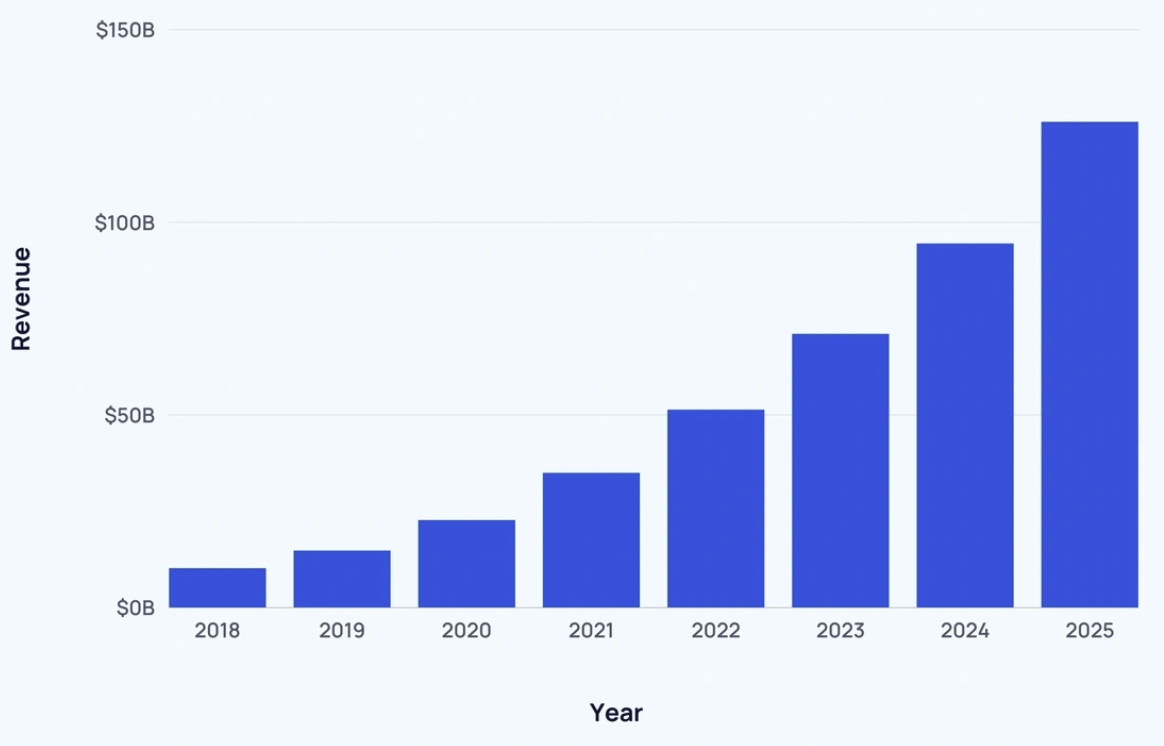
\includegraphics[scale=0.4]{img/revenue.png}
    \caption{Global artificial intelligence software market revenue (Omdia). }
    \label{fig:revenue}
  \end{figure}

  It is clear from these three examples that the power of AI can help us make critical decisions. However, to determine whether it is objective or not is another matter, and to explore this, we must first learn how a ML model \textit{learns}. 

  \subsection{Primer on Supervised and Unsupervised Learning}

    Machine learning at its core is simply divided into \textit{supervised learning}, which tries to predict a label or outcome from some given input, and \textit{unsupervised learning}, which tries to predict patterns in a group of unlabeled data.\footnote{There is a third paradigm called \textit{reinforcement learning}, but for conciseness, we will not include it here} 
    
    In supervised learning, machine learning models take in a dataset of the form 
    \begin{equation}
      \mathcal{D} = \{(x_1, y_1), (x_2, y_2), \ldots, (x_n, y_n) \}
    \end{equation}
    where $n$ represents the amount of samples that this dataset contains. While the samples are abstracted away as symbols, these variables can really take on any number of forms. For example, if we have a dataset where we are trying to predict Airbnb prices given the number of bedrooms, number of bathrooms, and the average temperature in the area over the past year, then we have 
    \begin{equation}
      (x, y) = \begin{bmatrix} 3 \\ 2 \\ 67 \end{bmatrix}, \$123
    \end{equation}
    for a sample Airbnb listing that contains 3 bedrooms, 2 bathrooms, and an average temperature of 67 degrees Farenheit, with a listing price of \$123. The machine learning algorithm wants to find some function $f: \mathbb{R}^3 \rightarrow \mathbb{R}$ parameterized by some variables, and it does it by defining some cost function that determine how ``off'' the current function $f$ is from the true labels $y$. For example, the most commonly used loss function is the \textit{mean-squared error}, defined 
    \begin{equation}
      L(f) = \sum_{i=1}^n \big( y_i - f(x_i)\big)^2
    \end{equation}
    which essentially say that if we have some function $f$, and we try to predict the labels $\hat{y}_i = f(x_i)$, then the measure of how ``off'' it is from the true labels are the sum of the squared differences. Optimizing this algorithm essentially leads to our best predictor $\hat{f}$. 

    For unsupervised learning, we want to detect patterns in the data, which can be done through a loss function or some other optimization algorithm. The methods vary significantly, but we will list some here: 
    \begin{enumerate}
      \item If we were to find that there is not much correlation between the temperature and the listing price, then we can try to have a ML algorithm detect this for us. This is called \textit{dimensionality reduction}. 
      \item If we wanted to find some clusters where there are a lot of concentrated data points, we can use a \textit{clustering} algorithm. 
      \item If we wanted to see the overall pattern of how the data may have been generated or distributed, then we call this a \textit{density estimation} procedure. 
    \end{enumerate}

    Ultimately, without getting too much into the technicalities, the final predictor or result of our algorithm will be heavily dependent on two things: 
    \begin{enumerate}
      \item What form should our function be when learning? Should we restrict ourselves to linear functions? 
      \item What kind of data should we train it on? 
    \end{enumerate}
    These two questions heavily impact what the final result of our learning process will be. 

  \subsection{The Deep Learning Era} 

    Let us focus on the \textit{form}, more commonly referred to as the \textit{architecture}, of our function and what it means to paramaterize it. Going back to our previous Airbnb example, we may try to construct a simple \textit{linear predictor} that takes the form 
    \begin{equation}
      f(x) = \omega_0 + \omega_1 x_1 + \omega_2 x_2 + \omega_3 x_3 
    \end{equation}
    Essentially, we want to predict the listing price as a weighted sum of the input features, and essentially we are looking for the best possible combination of numbers $\omega = (\omega_1, \omega_2, \omega_3)$ that would predict the best (which is again done by minimizing our loss function). However, whatever our optimal parameter $\omega$ will be, we are always restricted to the set of linear functions. One may consider a more complex class of functions like all second-degree (and below polynomials) of the form 
    \begin{equation}
      f(x) = \omega_0 + \omega_1 x_1 + \omega_2 x_2 + \omega_3 x_3 + \omega_{12} x_1 x_2 + \omega_{13} x_1 x_3 + \omega_{23} x_2 x_3 + \omega_{11} x_1^2 + \omega_{22} x_2^2 + \omega_{33} x^3
    \end{equation}
    which is now a 10 parameter class of functions, and our job now is to optimize the best 10-valued $\omega$. As we increase our number of parameters, our function can become more ``flexible'' to capture a greater number of functions that may capture the pattern in the data.\footnote{This introduces another problem called overfitting, which is seen almost everywhere in machine learning, but since it is only loosely relevant to our ethical analysis of black-box AI, it will not be included in here.} Modern CPUs and GPUs have overcome the computational cost of adding more parameters through clever and large-scale hardware that uses \textit{parallelization}, the act of computing large scale problems in parallel. Combined with clever techniques, called backpropagation, to optimize these parameters over extremely high-dimensional spaces (i.e. over a large number of parameters), these developments paved the way for \textit{deep neural networks} to take over. 

    Deep learning refers to a subcategory of machine learning where researchers use deep neural networks as the model to optimize. It essentially refers to creating an extremely overparameterized model where $\omega$ may consist of millions or billions of parameters and training that over some data.\footnote{For those familiar with overfitting, it turns out that mysteriously, the overparameterization does not adversely affect the generalization capabilities of trained models. The reason for this is still not completely understood. } Inspired by the structure of the brain, the specific architecture of these models, consist of a composition of linear maps (matrices) resembling the interconnectedness of neurons, followed by a nonlinear \textit{activation layer} resembling how electric impulses are run through action potentials.  

    Deep learning has been very successful in recent years, and has been used to achieve state-of-the-art performance on a wide range of tasks, including image recognition, speech recognition, and natural language processing. One of the key advantages of deep learning is its overparameterization, which allows it to automatically learn features from the data and can be very useful when the features are complex and difficult to hand-engineer. For example, in image recognition, deep learning algorithms can automatically learn features such as edges, textures, and shapes from the raw pixel data, which can be used to classify the images into different categories.
    
    One of the first notable examples is AlphaGo, developed by Google's DeepMind. AlphaGo's victory over Lee Sedol, a world champion Go player, in March 2016 marked a significant milestone in the application of deep learning \cite{alphago}. Traditional algorithms in Go relied on manually crafted rules and heuristics to evaluate board positions and predict moves. These classical approaches, while effective to a degree, struggled with the immense complexity and vast number of possible positions in Go—a challenge that exponentially surpasses that of chess. Deep learning, by contrast, approaches this problem through neural networks that learn to recognize patterns and evaluate board positions by processing data from thousands of amateur and professional games. AlphaGo included a combination of deep convolutional neural networks and reinforcement learning, where the system learned winning strategies by playing millions of games against itself, constantly learning and adapting strategies without human input. This self-learning capability enabled AlphaGo to uncover novel strategies and insights that had not been explored by human players.

    Deep learning has also fundamentally shifted the field of computer vision, beginning around 2012 when a deep neural network named AlexNet dramatically outperformed classical image processing models in the ImageNet Large Scale Visual Recognition Challenge, a competition that tasks algorithms with classifying images into 1000 different categories \cite{alexnet}. Following the success of AlexNet, the use of deep convolutional neural networks (CNNs) became the standard in computer vision tasks. These networks excel in tasks ranging from image classification to object detection and image generation, leveraging layers of interconnected nodes that mimic the human brain's ability to process visual data. Several variants of CNNs have been developed since AlexNet, ranging from deeper architectures like GoogLeNet, ResNet, and Vision Transformers (ViTs) with a wide variety of applications in object detection (YOLO) and real-time object tracking (Omni-Scale Net) \cite{lenet, resnet, vit, yolo, osnet}. These models have achieved remarkable performance in image recognition tasks, often surpassing human accuracy on benchmark datasets.

    \begin{figure}[H]
      \centering 
      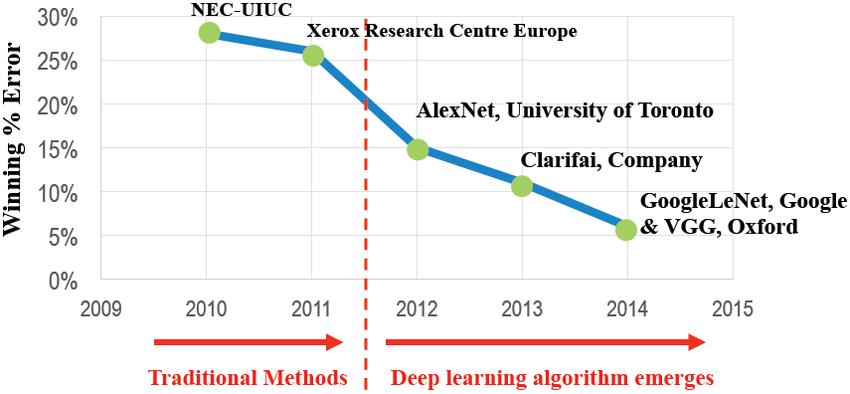
\includegraphics[scale=0.4]{img/imagenet.png}
      \caption{Up until 2011, traditional methods with moderately parameterized models have been state of the art when predicting labels in the ImageNet dataset. However, since the development of neural networks, they have greatly surpassed classical models \cite{imagenet}.} 
      \label{fig:imagenet}
    \end{figure}

    The supremacy of these complex models have spread a common belief throughout the research community that there is an inherent tradeoff between simplicity and accuracy. With simple traditional models, there is ultimately a plateau where patterns in the real world become to complex for them to detect. Therefore, complex models is a necessity for modern performance, even at the cost of simplicity and complete understanding of these models. 

  \subsection{Black Box Nature of Neural Networks}

    One of the key challenges in understanding and interpreting deep learning models lies in their overparameterization. Unlike simpler models like linear regression, where the weights of the weighted sum directly represent the importance of each feature in determining the final output, the weights in deep neural networks are not easily interpretable. The sheer number of parameters in these models, often in the millions or billions, makes it virtually impossible to ascertain the meaning or significance of each individual weight. This lack of interpretability is a major drawback, as it hinders our ability to understand how the model arrives at its predictions and to identify potential sources of bias.

    Moreover, the features learned by deep neural networks are themselves not interpretable. While there have been efforts to visualize and understand what the model is learning, such as activation maps that highlight regions with high weights, these techniques often produce noisy and inconclusive results \cite{gradcam}. The abstract nature of the features learned by the model, particularly in the deeper layers, makes it challenging to assign any human-understandable meaning to them. This lack of feature interpretability further compounds the difficulty in explaining the model's decisions and identifying the factors that influence its predictions.

    \begin{figure}[H]
      \centering 
      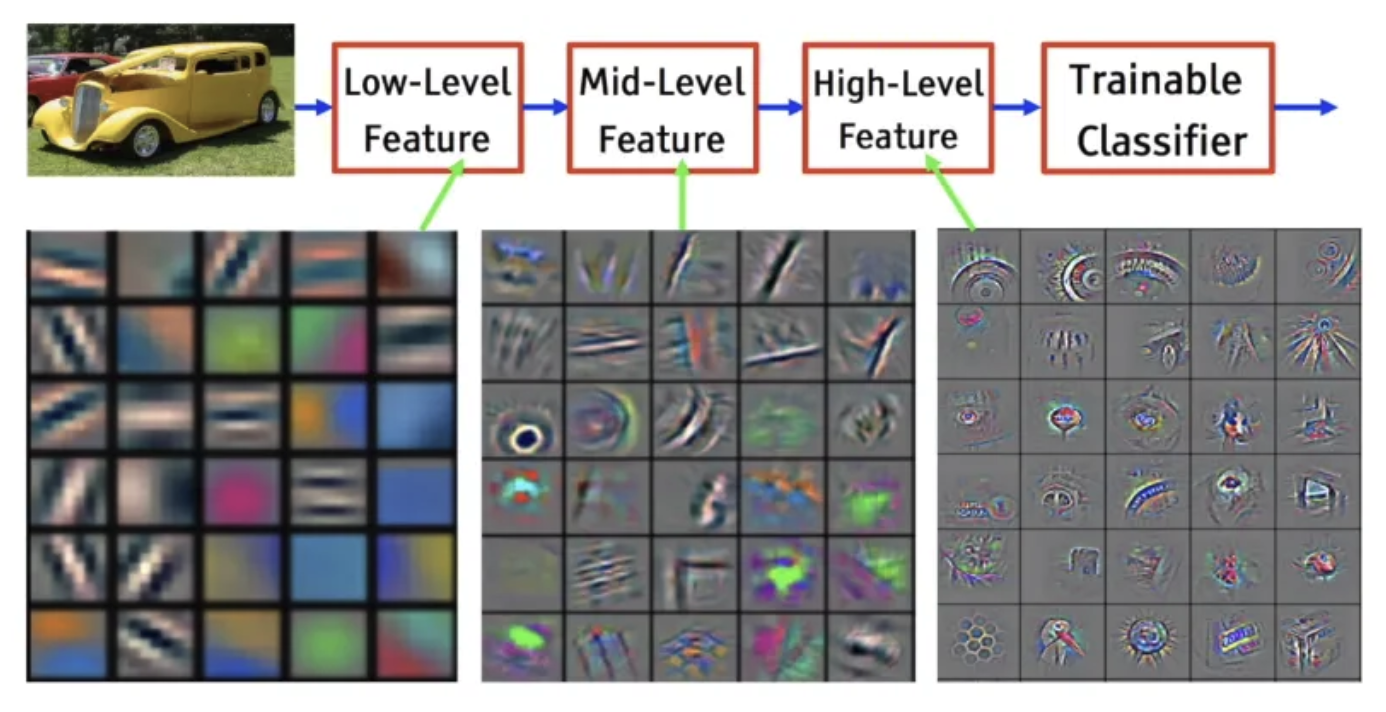
\includegraphics[scale=0.4]{img/features.png}
      \caption{From looking at the outputs of neural networks in their intermediate layers, it is difficult to really interpret which features that the model is using or not \cite{cnn}. Humans have a very coarse idea of how the neural network actually interprets this data.} 
      \label{fig:features}
    \end{figure}

    Furthermore, the fact that these aren't interpretable greatly reduces the ability of humans to mitigate potential errors that these models may make. If humans were to look at a traditional linear model and see a wrong prediction, they can point to a certain input $x_i$ and its corresponding weight $\omega_i$ and claim that this misweighting was the reason for the error. For neural networks, this is highly nontrivial to even identify which of the billions of weights were wrong. In fact, this has even led to the emergence of the field of adversarial attacks, which exploits the lack of interpretability by making small, imperceptible changes to the input that cause the model to make vastly incorrect predictions \cite{adversarial}. These attacks highlight the vulnerability of deep learning models and the need for more interpretable and robust approaches.

    \begin{figure}[H]
      \centering 
      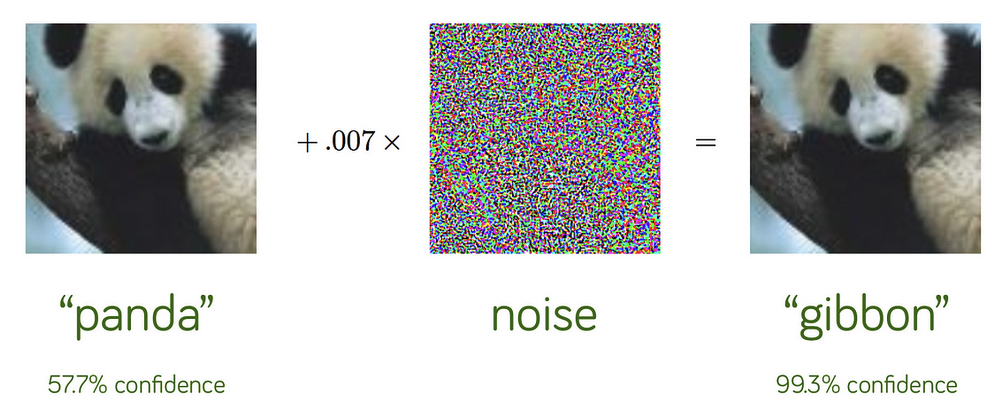
\includegraphics[scale=0.6]{img/adversarial.png}
      \caption{Adding a carefully chosen small perturbation to the input data of a panda causes a fully optimized neural network to predict it as a \textit{gibbon} with 99.3\% confidence. This represents the instability of these neural nets and more importantly, it is not clear how to fix these weights. } 
      \label{fig:adversarial}
    \end{figure}

    Clearly, this raises many eyebrows on the power and robustness of AI, especially since we rely so heavily on them for critical decision making. 

\section{Ethical Dilemmas and Sources of Bias} 

  The instability and non-interpretability of neural networks is a significant concern that the majority of consumers are not aware of. A severe consequence of blindly training these models can lead to \textit{algorithmic bias}, which occurs when algorithms make decisions that systematically disadvantage certain groups of people. Let us explore how this bias can occur. Recall that the two main factors that govern the performance of a model is its architecture and the data that it is trained on. A badly chosen dataset or architecture can induce or even exacerbate bias into the model. 

  \subsection{Dataset-Induced Bias}

    When we train a ML model with a dataset $\mathcal{D} = \{(x_i, y_i)\}$, we are essentially having it copy the structure of the dataset as much as it can by encoding it in the parameters. However, this is trained under the assumption that the integrity of the dataset is uncompromised, which may not be the case. Ultimately, it is humans that construct these datasets, and we may perpetuate our biases into them as well when collecting data or labelling them. For example, if a dataset used to train a hiring recommendation system predominantly consists of successful male candidates, the model may learn to associate male gender with better job performance, leading to discriminatory outcomes. 

    One prime example of an unethical dataset that was later detected to be unethical was the \textit{Boston Housing Dataset}, a dataset that collected information on 1978 housing prices in Boston in relation to several factors \cite{boston} However, one of the main ethical issues was the presence of racial bias. The dataset included a feature called \texttt{B}, which represented the proportion of Black residents in each area, which has been severely criticized for its potential perpetuate racial stereotypes and discriminatory practices in housing. It has been shown that models that were trained on this dataset had learned to associate lower housing prices with areas having a higher proportion of Black residents, which led to severe algorithmic bias. 

    Through this example, the inclusion of certain features that humans may, at the time, deem relevant to a certain indicator, may be a manifestation of an implicit bias that they project onto the dataset. A common theme in statistics, these biases can form in multiple ways. 
    \begin{enumerate}
      \item \textbf{Historical bias}: Many datasets reflect historical inequalities and societal biases. Using such data to train models can reinforce and perpetuate these biases.

      \item \textbf{Selection bias}: The process of collecting and curating data can introduce bias if certain groups are over- or under-represented in the dataset. This may just be a result of the availability of data, but researchers may not have the time nor the resources to collect balanced datasets. There is a field of statistics that deal with imbalanced dataset, e.g. when a dataset consists of, say 90\% males vs 10\% females. 

      \item \textbf{Measurement bias}: The way data is collected and labeled can also introduce bias. For example, if the criteria for labeling data are subjective or inconsistent, it can lead to biased outcomes. This can happen when humans try to label data, especially at a large scale. Furthermore, in the realm of semi-supervised  or weakly-supervised training, these models. 

      \item \textbf{Temporal bias}: Datasets may become outdated over time, leading to models that do not reflect current realities or societal changes. Organizations may use models trained on historical data that may not be relevant to current days, leading to inaccurate representation of certain groups of people.  
    \end{enumerate}

    To mitigate dataset-induced bias, it is crucial to carefully examine the data used for training, ensuring that it is representative, diverse, and free from historical or societal biases. Techniques such as data balancing, stratified sampling, and bias detection algorithms can help identify and address these issues.

  \subsection{Architecture-Induced Bias}

    The choice of the model architecture can be just as important when detecting bias in a system. Going back to the linear model example, with 3 variables, say $x_1, x_2, x_3$. 
    \begin{equation}
      f(x) = \omega_1 x_1 + \omega_2 x_2 + \omega_3 x_3
    \end{equation}
    Constructing a model of this form is really another assumption, where the designers think that the output label is really just dependent on a weighted combination of the inputs. Almost always, these assumptions are not well-justified, even though they may have good predictive power.\footnote{This leads to the saying that ``all models are wrong, but some are useful.''} However, other researchers may want to construct a different model in which there is a codependence relationship between $x_2$ and $x_3$, and they may add another parameter as such: 
    \begin{equation}
      f(x) = \omega_1 x_1 + \omega_2 x_2 + \omega_3 x_3 + \omega_{23} x_2 x_3
    \end{equation}
    The reasons for this extra term may depend on the researchers own experience, which again is prone to bias. This codependence assumption may be a great insight or biased opinion, but it is especially hard to determine within a lab environment where only a small team of researchers may be designing it. From this minimal example, we can see that in neural networks, it is not just one or two parameters, but the shifting-around, restructuring, and addition of millions of parameters that can severely affect the form of the final predictor. Even worse, these changes, however, major, are not as straightforward to detect as simply adding a codependence term like we did in the linear model due to the black-box nature of neural networks. 

    One more effect that we have not mentioned was the specific choice of the loss function, which can be considered as contained within our model assumptions. For example, consider a model that attempts to predict whether an individual is pro-abortion or pro-life, but the dataset consists of 90\% males and 10\% females. Using a generic mean squared error loss (or more commonly used cross-entropy loss) that takes an average of all the errors will underrepresent women's opinions on the matter. A more sophisticated loss function that takes this into account will be needed, along with more unbiased metrics such as the \textit{balanced accuracy} rather than just accuracy. 

    Ultimately, to address architecture-induced bias, it is essential to carefully design and validate the model architecture, considering factors such as model complexity, fairness objectives, and robustness to different types of data. There is a library of techniques like regularization, cross-validation, and fairness-aware learning algorithms can help mitigate bias and ensure more equitable outcomes, but more fundamentally, researchers must take caution to really identify which biases their assumptions may contain before training a model. 

\section{Case Studies: Addressing Socio-Economic Bias}

  Algorithmic bias in socio-economic factors is pervasive across critical fields such as healthcare, government programs, education, credit and finance, and housing and development. The widespread incidence of such biases in essential areas that shape our daily lives highlights the reality that anyone could be at risk of experiencing algorithmic bias at any time. This situation calls for an urgent need to develop methods to detect and mitigate these biases before they impact individuals, urging a proactive approach to safeguard fairness and equity in the application of AI technologies.
  \begin{enumerate}
    \item Healthcare: In a study that investigates the impact of socioeconomic status on the performance of AI models using electronic health records to predict asthma exacerbations in children, it was revealed that the lower socioeconomic status, measured by housing-based socioeconomic status index, correlates with higher balanced error rates in predictive models \cite{juhn2022assessing}. This suggests that AI models may perform worse for individuals from lower socioeconomic backgrounds , likely due to incomplete or inaccurate EHR data. This study highlights critical concerns regarding algorithmic bias in healthcare, particularly how AI models can inadvertently depend the healthcare disparities by performing poorly for underprivileged socioeconomic groups. The socioeconomic biases in AI tools can lead to worse health outcomes for these populations, and therefore, this study emphasizes the need of integrating socioeconomic indicators into AI model development and testing. 
    \item Government programs: The MiDAS algorithm employed by Michigan from 2013 to 2015 serves as a stark example of how algorithmic bias can pervade government programs, leading to substantial socio-economic consequences for individuals. This automated system was designed to detect fraud in unemployment claims but instead erroneously accused over 40,000 people of fraudulent activity. This failure resulted from a lack of human oversight and the algorithm’s reliance on defective data, leading to wrongful accusations that caused severe financial distress, including heavy fines, bankruptcies, and even home foreclosures. The appeals process later revealed a mere 8\% uphold rate for the algorithm’s decisions, highlighting its significant inaccuracies and unfairness. The public outcry that followed these revelations led to legal challenges and a critical audit, emphasizing the urgent need for transparency, accountability, and proper human monitoring in the deployment of algorithmic solutions in sensitive public sectors. This case illustrates the potential dangers of unchecked automated systems and the importance of implementing robust safeguards to protect individuals from erroneous algorithmic decisions that can have life-altering effects.
    \item Education: In 2020, the cancellation of final exams across England due to the COVID-19 pandemic presented significant challenges in grading and college placements for students. To address this, the Office of Qualifications and Examinations Regulation (Ofqual) deployed an algorithm designed to estimate student grades. This algorithm incorporated factors such as teacher predictions, individual student performance, and the historical performance data of each school. However, it soon became evident that the algorithm was biased, disproportionately lowering the grades of 40\% of students, especially those from lower-income backgrounds or attending larger public schools, compared to their counterparts in smaller, private institutions. This disparity triggered a massive public outcry, reflecting deep concerns about fairness and equality in educational opportunities. Critics argued that relying on historical school data perpetuated existing inequalities, as schools with historically lower performance, often in less affluent areas, were systematically disadvantaged by the algorithm. IIn response to the backlash, Ofqual made the decision to discard the algorithm-generated grades and revert to the original grades assigned by teachers, acknowledging the flaws in the automated system. This case serves as a cautionary example about the potential unintended consequences of relying on algorithms for decision-making in the education sector and the need to ensure equity and fairness in their outcomes.
    \item Credit and Finance: The credit and finance sector has experienced significant challenges related to algorithmic bias, particularly in how data brokers and payday lenders target vulnerable populations. For instance, during the coronavirus pandemic, payday lenders were reported to specifically target those financially impacted by the crisis, capitalizing on their urgent need for cash \cite{jones2020payday}. This practice often leads to high interest rates and traps consumers in cycles of debt. Additionally, a report by the United States Senate Committee on Commerce, Science, and Transportation in 2013 highlighted the role of data brokers in the collection, use, and sale of consumer data for marketing purposes. These activities often lack transparency and can lead to biased decision-making in credit scoring and financial services. The use of consumer data without explicit consumer knowledge or consent further exacerbates issues of fairness and equity in financial services, affecting credit opportunities and financial health of the most vulnerable populations. Both cases underscore the urgent need for regulatory scrutiny and the implementation of fairness and transparency guidelines to prevent algorithmic biases in financial decision-making processes.
    \item Price optimization: The Princeton Review, an established educational service provider, faced scrutiny when its pricing algorithm for the Premier SAT course—ranging between $6,600 and $8,400—was analyzed by ProPublica. The investigation revealed that this algorithm was not solely based on geographic cost differentials or standard business factors. Instead, ZIP codes characterized by higher median incomes and significant Asian-American populations were systematically quoted higher prices. Remarkably, neighborhoods predominantly inhabited by Asian-Americans were nearly twice as likely to receive these higher quotes compared to other groups, including in instances where these areas were not high-income. This pricing strategy raises serious concerns about fairness and discrimination in algorithmic decision-making. This example of differential pricing, also referred to as price optimization, highlights the complexities and potential biases embedded within algorithms used in commercial applications. The findings suggest that algorithms, while often perceived as neutral tools, can perpetuate or even exacerbate existing social inequalities. This is particularly concerning in sectors like education, where access to resources like tutoring can significantly influence a student's academic trajectory and future opportunities. The implications of such a case are profound, urging businesses and regulators alike to consider more stringent measures for transparency and fairness in algorithmic pricing. Ensuring that pricing algorithms do not inadvertently discriminate against any customer group not only aligns with ethical business practices but also protects the company from legal risks associated with discrimination. Furthermore, this situation emphasizes the importance of incorporating ethical considerations in the design and implementation of algorithms to prevent biases that can harm particular demographic groups.
  \end{enumerate}

  The case studies on algorithmic bias, spanning sectors from healthcare to education and government programs, highlight a pervasive issue: the influence of socio-economic factors on algorithmic decisions. These cases illustrate how biases in algorithms can exacerbate existing social inequalities, affecting everything from healthcare outcomes in lower socio-economic groups to educational opportunities and financial stability. Each example underscores the crucial need for integrating fairness and transparency in algorithmic design and implementation, advocating for regulations that ensure algorithms do not perpetuate socio-economic disparities. Addressing these biases requires concerted efforts from developers, policymakers, and stakeholders to revise and regulate the use of AI systems, ensuring they serve to enhance societal welfare rather than detract from it.

\section{Case Studies: Addressing Gender and Racial Bias}

  In this course, we had the opportunity to analyze the critical work of Joy Buluwami in understanding the inherent bias in many existing AI models. In particular, Buluwami’s work revealed that many of the commercial facial recognition techniques had inadequate detection for specific genders and races. Since then, research has found that one of the core reasons for bias in many state-of-the-art blackbox facial recognition models is training data \cite{sham2023ethical}. When populations are over or under-represented in training data or evaluation functions don’t take into account the imbalance in data, the models become unable to properly learn a variety of faces. As Buluwami states, “data is destiny.” In her thesis work, she found that error for identifying dark skinned females could be as bad as 47\%, nearly a coin toss’ chance \cite{buolamwini2024examining}.

  The danger of bias is not just a matter of facial recognition working or not working for certain people. The real danger is that these untested and unreliable technologies have already made their way into high impact use cases, such as hiring employees, identifying criminals in city streets, or calculating who is likely to default on a loan. One particularly notable example is the COMPAS algorithm, a proprietary recidivism algorithm developed in 1998 and implemented in US courtrooms as early as 2000 \cite{taylor2020ai}. This algorithm aims to expedite the process for predicting how at-risk individuals are to reoffend or be arrested after release. In principle, this is a promising idea. In fact, a 2017 study by the National Bureau of Economic Research on historical crime and judicial data found that machine learning techniques (in particular gradient-boosted decision trees) could theoretically aid in reducing crime rates up to 24.8\% without increasing incarceration rates, or conversely reduce incarceration by 42\% with no increase in crime rates \cite{kleinberg2018human}. However, COMPAS has remained a point of contention due to its proprietary nature. While COMPAS is presumed to follow legal regulation, such as not including race in its decision, it is completely unknown how COMPAS evaluates specific input variables. COMPAS was the source of controversy in 2016 when a ProPublica analysis of the algorithm revealed that COMPAS presented significant racial bias, and would often prescribe higher risk values to black individuals than white. Their results on Florida crime information showed that COMPAS was nearly twice as likely to rate black defendants who did not re-offend as “higher risk” compared to white defendants \cite{angwin2016machine}. But since COMPAS does not consider race, clearly the issue was not from direct racial bias. In fact, later analysis of the same study found that the underlying issue was that sampling of data itself was skewed. In particular, the Broward County data that was used had an over 10\% higher amount of black defendants who were rearrested, and consequently COMPAS showed predicted higher rates of reoffending without having seen race \cite{hao2019can}. In fact, Hao and Stray show that in order to achieve truly “equal” treatment between the white and black defendants from the data, the decision threshold for both races would need to be set at different levels, in effect requiring a racially biased decision in order to achieve a racially unbiased outcome.

  Clearly, addressing issues of bias in algorithms is not as simple as just designing better algorithms. In an issue of the Yale Law Journal, Sandra Mayson titles her article “Bias In, Bias Out,” and details how risk assessment algorithms display bias that exists as a result of a “racially stratified world,” and simply reproduces the existing bias which already exists in our societies \cite{mayson2019bias}. In particular, addressing gender, racial, or any other kind of algorithmic bias requires a twofold effort: firstly, in addressing bias in existing systems through more extensive analysis of data and identifying weakpoints; secondly, in addressing the opaque nature of black-box models. The first of these has been addressed by many groups through reinforcing data sets with more diverse samples and by doing post-hoc analysis on algorithmic bias. However, the second remains an under-researched issue for the most part. Black-box models are notoriously difficult to pierce, and proprietary technology like COMPAS makes it much more difficult to know why decisions are made. A study by Duke professors suggests that existing research already points to simple and publicly accessible models on recidivism performing as good as black box methods, while retaining a much higher degree of interpretability \cite{rudin2018age}. Yet, in many domains, black-box methods remain as the most accurate and commonly implemented. 

\section{Regulatory and Legal Frameworks to Combat AI Bias}

  While the aforementioned practices pave the way for more ethical AI, they only serve as guidelines, and cannot be enforced as strict rules. In fact, restricting research to those guidelines could be detrimental to the general landscape of AI research. To achieve effective regulation, we desire restrictions which only serve to protect the people, without stifling the pace of progress.

  As of now, there is a shocking lack of regulation and precedent to handle AI bias in the world. Since the explosion of AI, it has slowly found its way into more and more public-facing applications. One example that is extremely pressing to college students is the increasing usage of AI in employee screening, which allegedly is being employed by nearly 80\% of employers, according to survey data from February 2022 \cite{gilbert2023eeoc}. Despite the clear reality that AI has been a major factor in hiring screening for years, the first AI bias hiring lawsuit was filed and settled in August of 2023, only a few months ago. In this lawsuit against an English tutoring service named iTutorGroup, applicants found that their applications were automatically rejected when containing older birth dates, which the Equal Employment Opportunity Commision (EEOC) found to be in violation of the Age Discrimination in Employment Act and forced the company to pay \$365,000 to over 200 applicants who were automatically rejected due to being over 40 years old \cite{gilbert2023eeoc}.

  Another landmark lawsuit appeared around the same time in the healthcare industry with UnitedHealthcare, the “largest health insurance provider in the US” \cite{laney2023ai}. UnitedHealthcare obtained NaviHealth in 2020, and utilized their nH Predict algorithm to deny healthcare coverage to elderly patients. Surprisingly, the lawsuit claims that around 90\% of the claims are reversed when appealed to federal judges \cite{laney2023ai}. This lawsuit again reveals a concerning pattern of companies adopting AI and using it for years under the radar due to a lack of consistent regulation or review for these new technologies.

  A core issue with looking solely at judicial precedent is that these lawsuits only reveal and treat the symptoms of AI bias. To truly address the issue of AI and AI biases, legal and regulatory frameworks need to be created to comprehensively review AI before it is placed in important places. In particular, legal and regulatory systems should aim to primarily protect people when AI reaches the wild. AI which seeks to make a significant impact on the world needs to be vetted and subject to protective measures which ensure the safety of the models, and the safety of those using the models. We present below a number of principles which we believe these kinds of legal and regulatory systems should adhere to:

  \subsection{Safety Vetting and Trial Studies}

    AI has exploded in popularity and been implemented in a variety of use cases with limited regulation. In certain domains, existing infrastructure protects individuals from using untested AI, such as the Digital Health Innovation Action Plan enacted by the FDA to certify digital and AI powered medical products. We propose that this kind of framework should be extended to other other AI products, such as Deepfakes, voice cloning, media synthesis, autonomous systems, etc. A vetting system which requires compliance with regulation can help identify dangers or bias in AI before they reach the market, and in the case of emergent use cases, the vetting system can be the first line of defense in deciding some of the key precedent and rulings which dictate the future of those products. On top of necessitating new systems be put in place by the government, this kind of regulation would also require a push in the study of XAI and generating new or more standardized methods to evaluate AI safety.

    While this kind of system is not in place yet, it is worth noting that the government is not turning a blind eye to the issue. In an executive order from October of last year, President Biden listed a variety of directives regarding AI and plans to regulate AI usage. The first of the listed actions is the following:

    \begin{center}
      \textit{Require that developers of the most powerful AI systems share their safety test results and other critical information with the U.S. government.\cite{whitehouse2023fact}}
    \end{center}

    The directive additionally notes that the government seeks to work with the National Institute of Standards and Technology to “develop standards, tools, and tests to help ensure that AI systems are safe, secure, and trustworthy”\cite{whitehouse2023fact}. Among other key points listed are addressing AI discrimination in renting, criminal justice, and healthcare.

    While the federal government clearly recognizes the need for such regulation, true action is being taken more often at the local level. For example, in July of last year, New York City enacted a law which would require any employer using AI or ML in hiring processes to have annually performed audits on their systems to ensure their tools are not biased or discriminatory. The law requires the audits be performed by third parties, which mitigates any internal conflict of interest, and additionally requires employers make the audit results publicly available \cite{kestenbaum2023nyc}.

  \subsection{Human Liability}

    In many AI powered systems, especially those which have a degree of decision making or autonomy, rulings on “fault” are still decidedly unclear. In some cases, rulings come down to simply setting a precedent using existing systems, such as how generative AI art ownership has broadly been given to the users of the tech. However, in semi or fully autonomous systems, these kinds of decisions are less clear. Autonomous and driverless cars currently have very little precedent on who exactly takes blame when these vehicles crash. We propose that the faults of AI should be attributed to people as much as possible, whether that means the operator of the tool or the designer and/or distributor of the tool. In combination with the above principle, this aims to turn AI issues into human issues, which have existing precedent. Additionally, forcing the fault onto people will force AI product designers to be much more cautious with designing safe products, and additionally force operators to be more careful and aware during use of AI tools.

    As of now, solutions towards AI liability are still nebulous and unexplored. For example, generative AI has become a hotbed of legal contention between corporations, users, and courts due to the unprecedented nature of their liability. As we alluded to, there has been much debate on copyright entitlement and infringement regarding AI content. However, more serious issues are also at play, such as liability of harmful AI generated content. Claims against ChatGPT performing defamation or Gemini being “too ‘woke’” have brought into question who should be at fault for the output of these models. A particularly relevant piece of legal protection comes from Section 230 of the Communications Decency Act, which more or less protects corporations from the content posted on their platforms by other individuals (for example Twitter is not liable for everything its users say). However, numerous legal experts from universities as well as Supreme Court Justice Neil Gorsuch argue that Section 230 should not protect AI content \cite{mims2024ai}. While corporations and courts may be in opposition on the matter, it remains unresolved.

    Though the US has not had strong statements or judicial cases regarding liability, the EU has begun taking steps towards AI liability that could serve as a powerful precedent. In their “Artificial Intelligence Liability Directive,” the European Parliamentary Research Service draws on prior regulation on “producers’ strict liability regime for defective products,” and notes the outdated nature of some of these paradigms due to the difficult burden of proof for AI systems. In their proposal, they seek to introduce a regime that would place liability of “high-risk AI system[s]” on the operator unless the operator is “able to prove that it has abided by its duty of care” \cite{ec2022artificial}. Revising existing product liability and enacting operator liability regulations could serve to clear up uncertainty regarding liability in AI systems, and generally falls in line with our proposed principles. Though this proposal has yet to make its way to implementation, the ideas proposed serve as a powerful reference for the future of the US with regards to AI liability.

    \begin{figure}[H]
      \centering 
      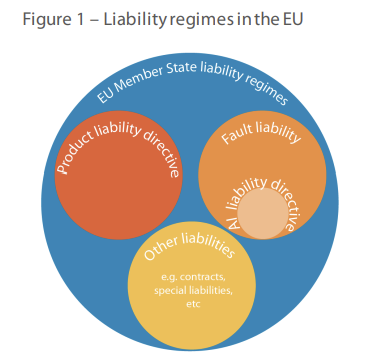
\includegraphics[scale=0.4]{img/liability.png}
      \caption{Source: European Commision 2022} 
      \label{fig:liability}
    \end{figure}

  \subsection{Flaw Acknowledgement}

    Though many people may misconceive AI to be superior or even infallible in comparison to people, this couldn’t be farther from the truth. In numerous cases, AI has failed because it is built by humans. In particular, AI is built on past data and thus is prone to replicate or even exacerbate existing biases in our world. In an era where AI is becoming increasingly prevalent, it is important to acknowledge its failings openly in order to open the door to improvement and safer operation. Acknowledging limitations will allow operators of AI powered tools to decide where and when human judgment should be used to monitor, modify, or supersede AI decisions.

    Addressing these kinds of flaws requires a more comprehensive study on the nature of AI issues. While we have discussed in our course the work of key figures like Joy Buolamwini in revealing biases in AI, the approach of manually identifying biases or waiting until third parties recognize issues is a only a post-hoc approach and can only recognize issues after models have made their way to products. Developing tools and techniques which standardize and simplify the issues of identifying bias is key to making a comprehensive study and theory regarding AI flaws. One half of the solution may be found in XAI, where a comprehensive study of why AI make the decisions they do may reveal underlying biases. For example, researchers studying the word2vec model found that the model learned gender-biased word associations, which revealed issues with the underlying training data as well as the model \cite{bolukbasi2016man}. The other half of the solution is building up better toolkits which can streamline the process of identifying biases. A number of tools exist for this purpose, primarily released by the largest corporations in the AI industry, such as IBM’s AI Fairness 360, Google and Tensorflow’s Fairness Indicators, and Microsoft Fairlearn. It is difficult to make a generic technique for bias in all domains, as it can be expressed in different models and datasets differently. Addressing this issue in full requires putting newfound research efforts into XAI and AI fairness.

    Following these principles has the potential to slow AI adoption and application, but also ensures that regulation can progress at a pace which matches the growth in use of AI. In particular, it explicitly forces AI designers to address inherent biases and flaws in their systems early on, and similarly forces governmental entities to take a stance on AI sooner rather than later.

    While AI research is relatively unaffected by these guiding principles (as they primarily are aimed at bringing AI to market), they may lead to a transition from a performance and outcome oriented approach to a more cautious and conscientious approach when handling industry AI research.

\section{Technological Solutions and Ethical Guidelines for AI Development}

  The regulatory perspective on mitigating the effects of AI bias may be effective, but there still remains technological concerns about the nature of AI research, and whether we ought to be cautious about the development of more powerful AI. While these fears in laypeople are no doubt spurred on in part by the plethora of media depicting sentient, dangerous AI, these fears are not without truth in the academic world. The petition for a 6-month pause on AI research following the release of GPT-4 was filled with high-profile researchers, politicians, and industry executives, many of whom work directly with AI, causing large-scale discourse amongst leaders in the machine learning community. From exploring and scrutinizing the norms and principles of machine learning research, we have determined 3 themes that must be strengthened and adhered to in order to ensure that the technological development of deep learning is directed towards an ethical direction. 

  \begin{enumerate}
    \item Visualization, simplification, and prototype networks. 
    \item Transparency in AI generated content.  
    \item Focus on development in neighboring fields. 
  \end{enumerate}

  \subsection{Visualization and Prototypes} 

    The most important factor in proceeding safely with AI research is transparency. Despite the extensive research in the field, black-box models still prove inscrutable and often unpredictable. Though less prominent than other niches of the field, interpretable AI or explainable AI (XAI) has increasingly been an area of focus in the AI world, especially after the unfulfilled petition for a 3-month halt on AI research after the announcement of ChatGPT. AI transparency has generally been split into two worlds: XAI, where post-hoc systems which seek to analyze black-box models in an understandable way (such as studying variable importance or white-box twinning), and interpretable AI which are models which, by design, are easy to understand (such as decision trees or ProtoPNet). Putting more effort in demystifying AI will allow us to better understand why AI bias occurs, and how we can most effectively address it.

    The concern of interpretability is not a new one. Since data processing and statistics have been used, it data analysts would make charts and graphs, which was essentially a way to reduce the complex data into some reasonable form. Extremely high-dimensional data such as market trends, economic prosperity, or the environmental state of the Earth has been narrowed down into specific key statistics such as the stock price of the S\&P 500 index, the GDP of a country, or the metric tons of $C O_2$ emissions per year. Humans have done a great job to reduce even the most complex data into numbers that they can manage. 

    This leads to the first component of our solution: visualization. It is clear that humans rely on visual data and thus we have spent great efforts to develop clever techniques when working with the complex or the abstract. Even in the early days of machine learning, scientists have plotted the decision boundaries of certain classifiers to see how an algorithm would classify inputs, heatmaps of different input feature to determine which ones were important to a decision, or even contour maps of a complex probability distribution. 

    When the effectiveness of neural networks were known, statisticians and machine learning researchers had focused too much on maximizing the predictive power of these algorithms rather than trying to interpret what they have meant. With the explosion of computer vision, the intrinsic visual nature of the image and video data pushed them to develop visualization techniques. This led to one of the most famous visualization techniques, known as \textit{saliency maps}, that generated a heatmap over the input data that highlighted parts of the input (such as pixels in image recognition tasks) that are most influential in determining the output \cite{cam}. This allowed researchers and developers to understand which features the model is actually paying attention to, being particularly useful in applications like medical imaging, where understanding the focal points of a model can confirm whether it is considering the clinically relevant areas in an image. 

    \begin{figure}[H]
      \centering 
      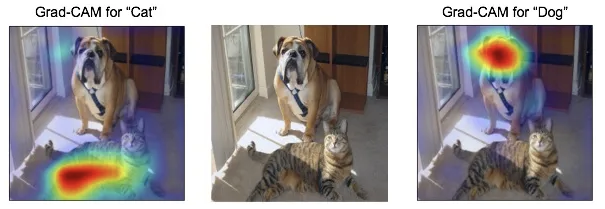
\includegraphics[scale=0.6]{img/gradcam.png}
      \caption{Grad-CAM is one of the most widely used kind of saliency map that allows researchers to visualize where a neural network is focusing on \cite{gradcam}. The original image is shown in the center, with the left image showing a heatmap over what the algorithm interprets a cat as, and the right image for that of the dog. } 
      \label{fig:gradcam}
    \end{figure}

    More recently, neural networks that use \textit{attention mechanisms} to deal with sequential data such as text or time-series, have provided a clearer picture of the internal workings of these models. More specifically, they show, by also generating some sort of heatmap, which parts of the input data are given more importance for predicting the next element in a sequence, or in other words, where the model has its attention on. This can be crucial for tasks like machine translation or sentiment analysis, where understanding the weight assigned to different words or phrases helps in fine-tuning the models and in verifying that the significant parts of the text are being considered appropriately. 

    Both saliency maps and attention mechanisms are extremely useful in providing good visualizations on either visual or sequential data, but another technique to increase interpretability is through \textit{Prototype Networks}, a model designed to enhance interpretability in image classification tasks developed by Dr. Cynthia Rudin of Duke University, a strong supporter of interpretable models. Prototype networks learn by utilizing specific image parts that represent key features of various classes, such as beaks and wings for birds, and wheels and windows for cars. During the training phase, ProtoPnet identifies these crucial features for each class it needs to distinguish between and then uses these prototypes as benchmarks to compare and classify new images by measuring how similar parts of the new image are to the stored prototypes.

    The core advantage of using ProtoPnet lies in its straightforward interpretability. Each decision made by the network can be directly traced back to visible, understandable parts of an image that the model deems most indicative of a particular class. This transparency allows users to see exactly why the network classifies an image in a certain way, by highlighting the parts of the image that activated the relevant prototypes. This method not only builds trust in the system's decisions but also makes it easier for users and developers to verify and improve the model's accuracy and fairness.

    In practical applications, such as medical diagnostics or autonomous driving systems, the ability to explain decisions becomes critically important. ProtoPnet's method of referencing clear, definable image features for decision-making allows it to provide justifications for its actions, enhancing user trust and compliance. This characteristic of ProtoPnet makes it highly valuable in fields where understanding the reasoning behind automated decisions is necessary for safety, ethics, or compliance reasons. Thus, ProtoPnet bridges the gap between achieving high performance in machine learning tasks and maintaining the transparency and interpretability needed in critical applications.

    By making it possible to trace how decisions are derived, interpretable models allow for a clearer delineation of responsibility among the various parties involved in the AI's lifecycle, from data collectors and model developers to end users. For example, if a model makes an incorrect or biased decision, it is possible to determine whether the error stemmed from biased training data, flawed model assumptions, or improper implementation. This clarity is vital in sectors like healthcare and criminal justice, where erroneous AI decisions can have severe consequences. 

  \subsection{Transparency in Research and AI Generated Content} 

    Even with the technology to provide great interpretable models and visualization to the broader network, there should still be a responsibility for the researchers and the users of these models. First, when scientists publish new works, there should be several standards of accountability practices that attempt to check and measure the biases in these new models. For example, ethical auditing where algorithms are systematically reviewed for bias, fairness, and ethical implications before deployment is crucial practice. This includes rigorous testing and validation of models on diverse datasets to ensure fairness and mitigate biases before deployment.

    It is of utmost importance that these publications should have as many professional eyes on it as possible. The research community should adopt a more open-source approach to facilitate greater collaboration and transparency. By making research papers, code, and datasets openly available, the community can collectively scrutinize and validate the findings, ensuring a more thorough examination of potential biases and unforeseen consequences. This open-source approach enables a diverse range of experts, including ethicists, social scientists, and domain specialists, to provide valuable insights and feedback. Moreover, it encourages the development of standardized frameworks and best practices for assessing the fairness and ethical implications of AI models. By fostering a culture of openness and collaboration, the research community can proactively identify and address potential issues before the models are widely deployed, thereby minimizing the risk of harmful consequences.

    Additionally, impact assessments, similar to environmental impact assessments, evaluate the potential consequences of deploying an AI system in real-world settings. These assessments are crucial for understanding the broader implications of AI technologies, including any negative impacts on certain populations. They provide a systematic framework for identifying and mitigating potential risks, such as unfair treatment, privacy violations, or unintended societal consequences. Impact assessments should involve a diverse range of stakeholders, including affected communities, domain experts, and policymakers, to ensure a comprehensive evaluation of the AI system's potential effects. By conducting thorough impact assessments and incorporating the findings into the development and deployment process, organizations can demonstrate their commitment to accountability and responsible AI practices. This proactive approach helps build trust with the public and ensures that AI systems are developed and deployed in a manner that prioritizes fairness, transparency, and the well-being of all individuals and communities involved.

    Transparency in AI content is also a key part of combatting misinformation and bias. A common method for images which is starting to be more widely adopted is the use of tagging AI generated content with C2PA metadata, which is an existing industry standard for media. However, C2PA metadata can easily be deleted and does not apply to text data. Designing a robust multimodal tagging system which can be verified, potentially utilizing elements of blockchain technology, would be a huge benefit in combating AI misinformation and bias. Not only can this address misinformation by providing clarity on what content is real and fake, it can also allow everyday users of AI learn to be more vigilant when viewing certain content to avoid being influenced by biased or altered information. Since AI content may replicate biases or hallucinate information unintentionally, knowing when content is AI generated is instrumental in keeping consumers of media aware of what flaws may arise in certain kinds of content.

    To further enhance the transparency and accountability of AI models, it is essential to establish comprehensive documentation practices and adhere to recognized standards for interpretable AI. This documentation should encompass all aspects of the AI system, including the data used, design and implementation choices, operational parameters, and any limitations or potential biases identified during the development process. By maintaining detailed records and providing clear explanations of the algorithms employed, we can facilitate a better understanding among non-expert stakeholders who may interact with or be affected by the AI system. Moreover, implementing a simple classification system, such as a flag that indicates whether the model has undergone ethical testing, can help users quickly assess the trustworthiness of the AI system. Regular updates to the documentation, as the model evolves and new data becomes available, ensure that the information remains relevant and accurate. By openly disclosing the capabilities and limitations of AI models, we can set realistic expectations and safeguard against potential misuse. The combination of interpretable architectures, advanced visualization techniques, and comprehensive documentation practices creates a solid foundation for building transparent and accountable AI systems that inspire trust and confidence among all stakeholders.

  \subsection{Advancing Research in Neighboring Fields}

    If we notice the most significant advances in artificial intelligence, they were all inspired by cross-domain knowledge in neighboring academic fields of study. Consider the following cases: 
    \begin{enumerate}
      \item When neural networks were first invented, they were inspired by the graph-like structure in the brain which fired electric impulses that are analogous to the activation functions used today in these algorithms. 
      \item The invention of the convolutional neural network was inspired by the idea of \textit{locality}, meaning that people tend to focus on specific regions of an image, and spatially close regions tend to correlate highly with each other than regions that are far apart. 
      \item The invention of the attention mechanism took the fact that individuals tend to focus on certain parts of an image or a sentence to derive meaningful conclusions, rather than just simply the pixels/words around it or the whole image/sentence at once. 
      \item The entire field of reinforcement learning is founded upon the idea of positive and negative reinforcement in psychology. 
    \end{enumerate}
    While these were the most popular, there are countless more contributions that were directed by some vague idea in another discipline, especially in neuroscience and psychology. The success of these breakthroughs are certainly correlated with the corresponding knowledge in related fields, leading to the suggestion that the best way to advance machine learning is to not focus on machine learning too much. Recent trends have shown that the overwhelming progress in deep learning had put too much focus in the statistics and quantitative metrics of everything. However, to ensure that this progress continues in a stable and responsible manner, it is crucial to recognize the importance of advancing research in neighboring fields such as neuroscience and psychology. By fostering a deeper understanding of the human brain and cognition, we can gain valuable insights that will guide the development of more robust, explainable, and ethically aligned AI systems. 

    Neuroscience research, which is still understood very little today and has plenty of room for progress, has the potential to shed light on the fundamental principles of information processing, learning, and decision-making in biological systems. By studying the intricate workings of the human brain, researchers can identify key mechanisms that can be adapted and incorporated into AI algorithms, causing more breakthroughs and at the same time gaining a deep understanding of the motivation behind these future architecture. This knowledge can lead to the development of more biologically plausible models that exhibit enhanced transparency, adaptability, and resilience. Moreover, insights from neuroscience can help address challenges such as catastrophic forgetting and few-shot learning, which are critical for creating AI systems that can learn continuously and efficiently, much like humans do.

    Similarly, advancements in psychology can provide a deeper understanding of human cognition, behavior, and social dynamics. By studying how humans perceive, interpret, and interact with the world around them, researchers can develop AI systems that are more attuned to human needs, preferences, and values. This interdisciplinary approach can lead to the creation of AI algorithms that exhibit greater emotional intelligence, empathy, and cultural sensitivity. Furthermore, insights from psychology can help in designing user interfaces and interaction paradigms that facilitate more natural and intuitive human-AI collaboration.

    In addition to neuroscience and psychology, there are several other fields that can contribute to the advancement of AI research. Sociology, for instance, can provide valuable insights into the complex social structures and dynamics that shape human behavior and decision-making. By understanding the societal factors that influence individual and collective actions, researchers can develop AI systems that are more socially aware and responsive to the needs of different communities. Similarly, economics and game theory can offer powerful tools for modeling and analyzing the strategic interactions between AI agents and human stakeholders, helping to design more stable and equitable systems that align with societal values and objectives.

    This flow of knowledge does not have to be one-way, either. The rigorous nature of quantitative studies can be greatly beneficial to the progress of some softer sciences, allowing scientists to get a better foothold of elusive ideas and theories not grounded in numbers. By fostering the interdisciplinary exchange of methods, tools, and perspectives, every field can inspire, validate, and benefit from each other. Ultimately, investing in research at the intersection of AI, neuroscience, and psychology will not only enhance the stability and robustness of machine learning algorithms but also ensure that the development of AI aligns with human values and promotes beneficial outcomes for society as a whole. 

\section{Conclusion}

\pagebreak

\bibliographystyle{IEEEtran}
\bibliography{./bibfile}

\end{document}
